% !TeX program = xelatex
% !TeX encoding = UTF-8
% !TeX TXS-program:compile = txs:///xelatex | txs:///xelatex
\documentclass[aspectratio=169, table, 12pt]{beamer}

% Preamble bersama seluruh slide mata kuliah ini.
% Dipanggil dari slides/sessionXX/sessionXX.tex tepat sesudah baris
% \documentclass[aspectratio=169, table, 12pt]{beamer}
% Paket tambahan yang hanya dibutuhkan satu sesi ditulis di berkas sesi itu.

\usepackage{colortbl}
\usepackage{xcolor}
\usepackage{listings}
\usepackage{tabularx}
\usepackage{booktabs}
\usepackage{tikz}
\usepackage{pgfplots}
\usepackage{fontspec}
\usepackage[english,bahasai]{babel}
\pgfplotsset{compat=1.18}
\usetikzlibrary{arrows.meta, positioning, calc, fit, shapes.geometric,
  shapes.multipart, backgrounds, matrix, chains, trees}

\makeatletter
\def\input@path{{../theme/}}
\makeatother
\graphicspath{{../theme/}{../../figures/}}
% Stub symlink Windows memakai tema cadangan sampai aset institusi tersedia.
\IfFileExists{../theme/beamerthemePradita.sty}{%
  \usetheme{Pradita}
}{%
  \usetheme{Madrid}
  \setmainfont{TeX Gyre Heros}
  \setsansfont{TeX Gyre Heros}
  \setbeamertemplate{navigation symbols}{}
}

\definecolor{praditagreen}{RGB}{37, 113, 71}
\setbeamercolor{structure}{fg=praditagreen}
\setbeamercolor{palette primary}{bg=praditagreen,fg=white}
\setbeamercolor{palette secondary}{bg=praditagreen!80!black,fg=white}
\setbeamercolor{palette tertiary}{bg=praditagreen!60!black,fg=white}
\setbeamerfont{frametitle}{size=\large}
\setbeamertemplate{caption}[numbered]

% Ukuran header mengikuti teks agar judul panjang tidak menabrak logo.
\setbeamercolor{frametitle}{bg=white,fg=black}
\setbeamertemplate{frametitle}{%
  \begin{beamercolorbox}[wd=\paperwidth,sep=0.2cm]{frametitle}
    \begin{minipage}[c]{0.77\paperwidth}
      \raggedright\fontsize{16}{18}\selectfont\bfseries\insertframetitle
      \ifx\insertframesubtitle\empty\else
        \par\small\mdseries\insertframesubtitle
      \fi
    \end{minipage}\hfill
    \begin{minipage}[c]{0.15\paperwidth}
      \IfFileExists{../theme/classFiles/logo_universitas.png}{%
        
\includegraphics[width=\linewidth]{../theme/classFiles/logo_universitas.png}%
      }{}
    \end{minipage}
  \end{beamercolorbox}
}
\setbeamertemplate{footline}{%
  \ifnum\value{framenumber}>1
    \begin{beamercolorbox}[wd=\paperwidth,ht=0.35cm,dp=0.15cm,
      leftskip=0.3cm,rightskip=0.3cm]{palette primary}
      \footnotesize\bfseries\insertframenumber/\inserttotalframenumber
      \hfill IT40513
    \end{beamercolorbox}
  \fi
}
\DeclareRobustCommand{\berkas}[1]{\path{#1}}

% Tema membuat garis tabel berwarna putih. Dikembalikan agar tabel terbaca.
\arrayrulecolor{black}
\setlength{\arrayrulewidth}{0.5pt}

\lstdefinelanguage{yaml}{
  basicstyle=\ttfamily\scriptsize,
  keywordstyle=\color{blue}\bfseries,
  commentstyle=\color{gray}\itshape,
  stringstyle=\color{red},
  showstringspaces=false,
  breaklines=true,
  frame=lines,
  numbers=none,
  backgroundcolor=\color{lightgray!10},
  tabsize=2,
  morecomment=[l]{\#}
}

\lstdefinelanguage{json}{
  basicstyle=\ttfamily\scriptsize,
  stringstyle=\color{red},
  commentstyle=\color{gray},
  breaklines=true,
  showstringspaces=false,
  tabsize=2,
  numbers=none,
  frame=lines,
  backgroundcolor=\color{lightgray!10},
  string=[s]{"}{"}
}

\lstdefinelanguage{bash}{
  keywords={},
  basicstyle=\ttfamily\scriptsize,
  ndkeywords={docker, kubectl, helm, curl, git, terraform},
  ndkeywordstyle=\color{purple}\bfseries,
  sensitive=true,
  commentstyle=\color{gray},
  numbers=none,
  breaklines=true,
  frame=lines,
  backgroundcolor=\color{lightgray!10},
  tabsize=2,
  comment=[l]{\#},
  showstringspaces=false
}

\lstdefinelanguage{http}{
  keywords={GET, POST, PUT, PATCH, DELETE, HEAD, OPTIONS, HTTP},
  basicstyle=\ttfamily\scriptsize,
  keywordstyle=\color{blue}\bfseries,
  sensitive=true,
  numbers=none,
  breaklines=true,
  frame=lines,
  backgroundcolor=\color{lightgray!10},
  tabsize=2,
  showstringspaces=false
}

\subtitle{IT40513 · Enterprise Architecture \& Digital Blueprint}
\author{\textbf{Alfa Yohannis}}


% Sampul membatasi judul di panel putih tema rujukan Pradita.
\setbeamertemplate{title page}{%
  \begin{tikzpicture}[remember picture,overlay]
    \node[anchor=north west,inner sep=0pt,text width=8.8cm]
      at ([xshift=1cm,yshift=-3.15cm]current page.north west) {%
        {\small\insertsubtitle\par}\vspace{0.25cm}
        \resizebox{8.8cm}{!}{\begin{minipage}{12cm}
          \raggedright\color{praditagreen}\bfseries\inserttitle
        \end{minipage}}
      };
    \node[anchor=south west,inner sep=0pt]
      at ([xshift=1cm,yshift=1.65cm]current page.south west)
      {\small\insertdate};
    \node[anchor=west,inner sep=0pt,text=white]
      at ([xshift=0.8cm,yshift=0.75cm]current page.south west)
      {\small\insertauthor};
  \end{tikzpicture}
}


% Batasi kedua dimensi gambar agar diagram bersama tetap berada pada slide.
\newsavebox{\eafigbox}
\newcommand{\eadiagram}[1]{%
  \sbox{\eafigbox}{\resizebox{0.94\textwidth}{!}{\input{#1}}}%
  \ifdim\dimexpr\ht\eafigbox+\dp\eafigbox\relax>0.64\textheight
    \resizebox{!}{0.64\textheight}{\usebox{\eafigbox}}%
  \else
    \usebox{\eafigbox}%
  \fi
}


\title{\Huge Gap Analysis\\ \vspace{10pt} dan Paket Kerja}
\date{Pertemuan 11}

\begin{document}

\begin{frame}
  \titlepage
\end{frame}

\begin{frame}
  \frametitle{Isi Pertemuan}
  \vspace{14pt}
  \begin{columns}[t]
    \column{0.5\textwidth}
    {\small\tableofcontents[sections={1-3}]}

    \column{0.5\textwidth}
    {\small\tableofcontents[sections={4-5}]}
  \end{columns}
\end{frame}

\begin{frame}{\hfill}
  \centering
  \Huge{\textbf{Bila rancangan target sudah\\disetujui, mengapa direksi\\belum tahu harus mulai\\dari mana?}}
\end{frame}

\section{Tujuan dan Konteks}

\begin{frame}{\hfill}
  \centering
  \Huge{\textbf{Tujuan dan Konteks}}
\end{frame}

\begin{frame}{{\Large Tujuan Pembelajaran}}
  \vspace{10pt}
  \begin{itemize}
    \item Menyusun \textit{gap analysis} lintas domain dengan membandingkan kondisi saat ini dan
          kondisi target.
    \item Mengelompokkan gap menjadi paket kerja (\textit{work package}) dengan ruang lingkup yang
          jelas.
    \item Menganalisis dependensi antarpaket kerja dan dampaknya pada pemangku kepentingan.
  \end{itemize}
\end{frame}

\begin{frame}{{\Large Masalah: Daftar Keinginan yang Rapi}}
  \vspace{10pt}
  \begin{itemize}
    \item Misalkan direktur keuangan bertanya: mana yang lebih dahulu, siapa penanggung jawabnya,
          dari mana tahu selesai?
    \item Kotak aplikasi baru tidak menjelaskan pembersihan identitas, pelatihan, kontrak, dan
          penghentian fungsi lama.
    \item Tanpa analisis selisih, peta jalan menjadi urutan pengadaan.
    \item Bab ini menjembatani C2 dengan rancangan target Bab 8 sampai Bab 10.
    \item Luaran sesi ini menutup tonggak C3 dan menjadi masukan Bab 12.
  \end{itemize}
\end{frame}

\begin{frame}{{\Large Diagram Konsep Bab 11}}
  \centering
  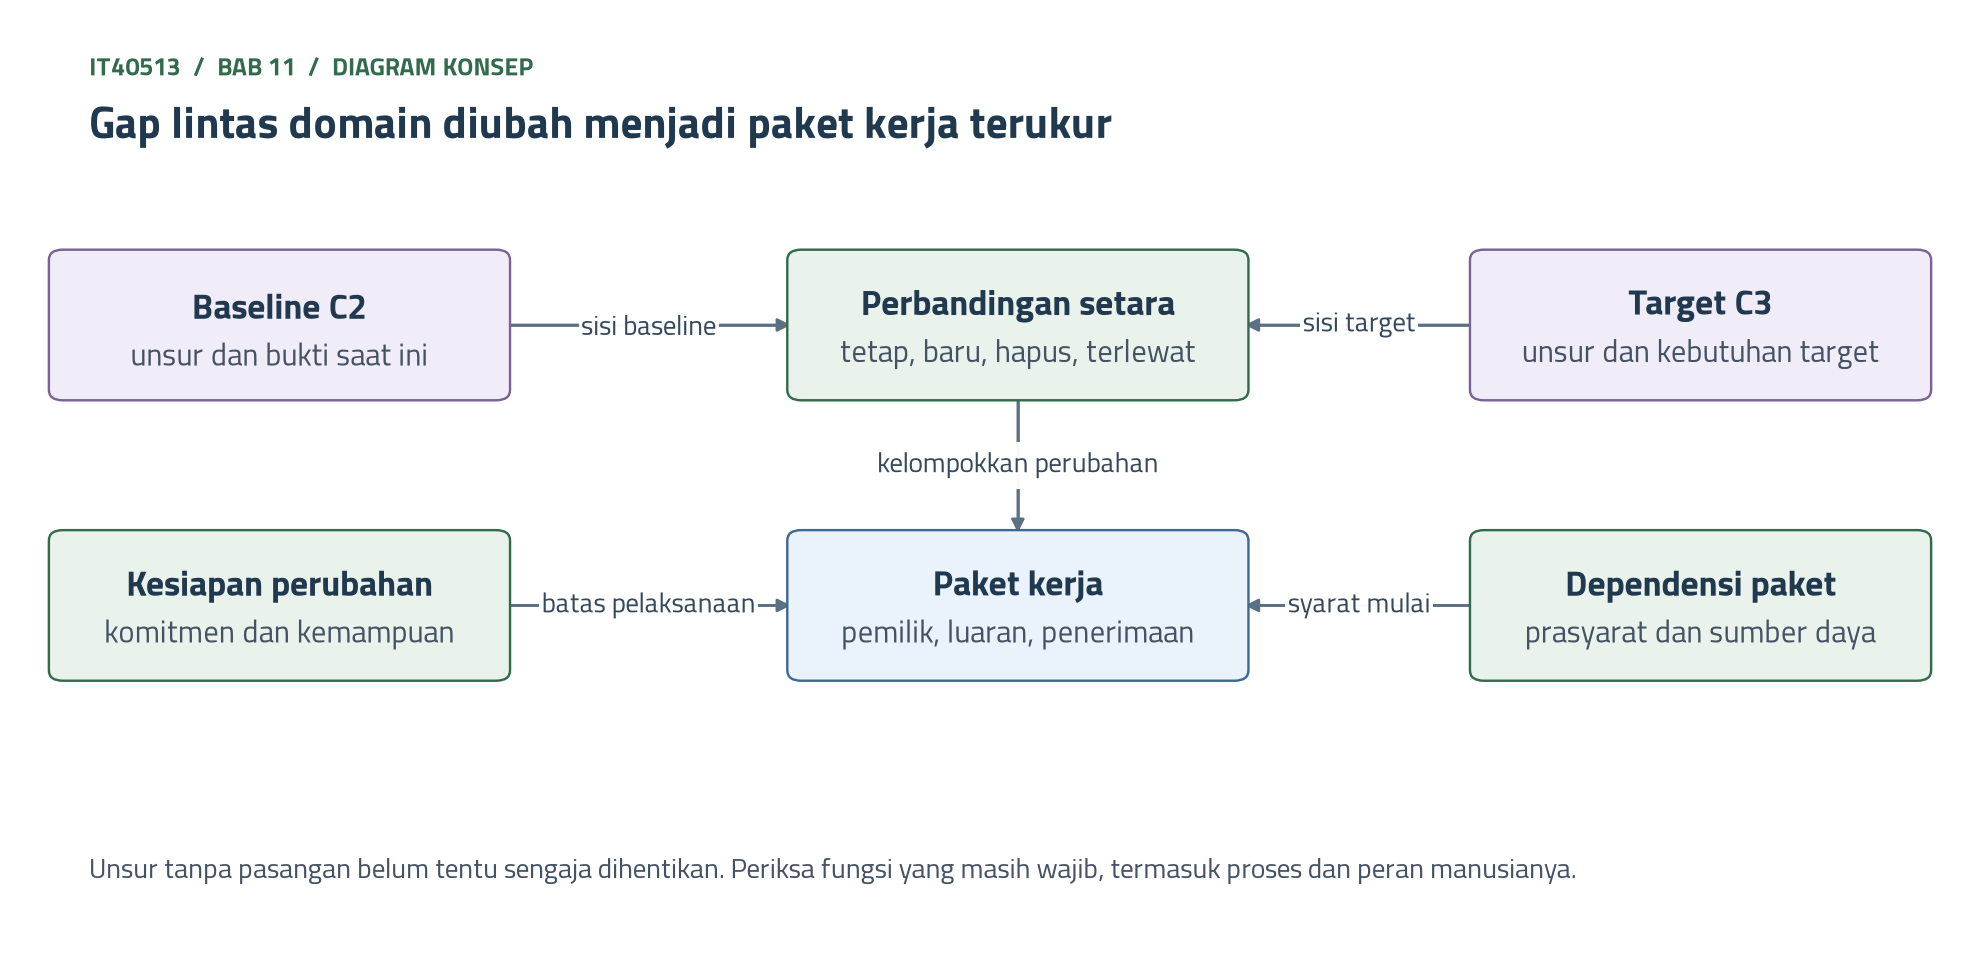
\includegraphics[width=0.96\textwidth,height=0.77\textheight,keepaspectratio]{../../figures/ch11-diagram-konsep.png}
  \label{fig:session11-ilustrasi-bab}
\end{frame}

\section{Gap Analysis}

\begin{frame}{\hfill}
  \centering
  \Huge{\textbf{Gap Analysis}}
\end{frame}

\begin{frame}{{\Large Teknik Gap Analysis dalam TOGAF}}
  \vspace{10pt}
  \begin{itemize}
    \item Membandingkan \textit{baseline} dan target pada lingkup yang sama.
    \item Memperlihatkan unsur yang sengaja dihilangkan, tidak sengaja terlewat, dan belum
          didefinisikan.
    \item Alatnya matriks: blok kondisi awal di sumbu tegak, blok target di sumbu datar.
    \item Ditambah satu baris \textit{New} dan satu kolom \textit{Eliminated}.
    \item Dikerjakan pada fase B, C, dan D ADM.
  \end{itemize}
  \vspace{6pt}
  {\small Analogi: pindah rumah. Lemari yang tidak ada di denah baru perlu keputusan: isinya
  dipindahkan ke mana?}
\end{frame}

\begin{frame}{{\Large Matriks Gap Medikara}}
  \centering
  \begin{figure}
    \resizebox{!}{0.76\textheight}{\begin{tikzpicture}[
  font=\scriptsize,
  kepala/.style={align=center, font=\tiny\bfseries},
  label/.style={anchor=west, align=left, font=\scriptsize},
  isi/.style={align=center, font=\tiny\bfseries}
]
  % Ukuran: kolom label 3,3 cm, delapan kolom masing-masing 1,08 cm,
  % baris judul 0,9 cm, sembilan baris isi masing-masing 0,66 cm.
  \fill[praditagreen!15] (0,0) rectangle (11.94,-0.9);

  % Sel berisi, diwarnai sebelum garis kisi digambar.
  \fill[green!10]  (3.30,-0.90) rectangle (4.38,-1.56);
  \fill[blue!8]    (4.38,-1.56) rectangle (5.46,-2.22);
  \fill[blue!8]    (4.38,-2.22) rectangle (5.46,-2.88);
  \fill[blue!8]    (5.46,-2.88) rectangle (6.54,-3.54);
  \fill[blue!8]    (6.54,-3.54) rectangle (7.62,-4.20);
  \fill[blue!8]    (7.62,-4.20) rectangle (8.70,-4.86);
  \fill[gray!35]   (10.86,-4.86) rectangle (11.94,-5.52);
  \fill[red!22]    (10.86,-5.52) rectangle (11.94,-6.18);
  \fill[orange!12] (8.70,-6.18) rectangle (9.78,-6.84);
  \fill[orange!12] (9.78,-6.18) rectangle (10.86,-6.84);

  % Garis kisi.
  \foreach \y in {0,-0.9,-1.56,-2.22,-2.88,-3.54,-4.20,-4.86,-5.52,-6.18,-6.84}
    \draw[gray!60] (0,\y) -- (11.94,\y);
  \foreach \x in {0,3.30,4.38,5.46,6.54,7.62,8.70,9.78,10.86,11.94}
    \draw[gray!60] (\x,0) -- (\x,-6.84);
  \draw[thick] (10.86,0) -- (10.86,-6.84);
  \draw[thick] (0,-6.18) -- (11.94,-6.18);

  % Judul kolom: elemen target, ditambah kolom Dihapus.
  \node[kepala] at (1.65,-0.45) {Baris: \textit{baseline}\\Kolom: target};
  \node[kepala] at (3.84,-0.45) {ERP\\keuangan};
  \node[kepala] at (4.92,-0.45) {SIMRS\\terpadu};
  \node[kepala] at (6.00,-0.45) {Platform\\integrasi};
  \node[kepala] at (7.08,-0.45) {Platform\\data};
  \node[kepala] at (8.16,-0.45) {\textit{Landing}\\\textit{zone}};
  \node[kepala] at (9.24,-0.45) {MPI};
  \node[kepala] at (10.32,-0.45) {Akses\\terpusat};
  \node[kepala] at (11.40,-0.45) {Dihapus};

  % Judul baris: elemen baseline, ditambah baris Baru.
  \node[label] at (0.08,-1.23) {ERP keuangan};
  \node[label] at (0.08,-1.89) {Lima SIMRS lokal};
  \node[label] at (0.08,-2.55) {SIM Klinik};
  \node[label] at (0.08,-3.21) {Integrasi \textit{point-to-point}};
  \node[label] at (0.08,-3.87) {23 laporan \textit{spreadsheet}};
  \node[label] at (0.08,-4.53) {Server lokal rumah sakit};
  \node[label] at (0.08,-5.19) {Antrean Bandung};
  \node[label] at (0.08,-5.85) {Surveilans infeksi Bogor};
  \node[label, font=\scriptsize\bfseries] at (0.08,-6.51) {Baru};

  % Isi sel.
  \node[isi] at (3.84,-1.23) {Tetap};
  \node[isi] at (4.92,-1.89) {Diganti};
  \node[isi] at (4.92,-2.55) {Digabung};
  \node[isi] at (6.00,-3.21) {Diganti};
  \node[isi] at (7.08,-3.87) {Diganti};
  \node[isi] at (8.16,-4.53) {Diganti};
  \node[isi] at (11.40,-5.19) {Sengaja};
  \node[isi] at (11.40,-5.85) {Tidak\\[-2pt]sengaja};
  \node[isi] at (9.24,-6.51) {Baru};
  \node[isi] at (10.32,-6.51) {Baru};

  % Keterangan.
  \node[font=\tiny, text width=11.8cm, align=center] at (5.97,-7.27)
    {Tetap: ada di kedua sisi. Diganti atau digabung: elemen lama punya padanan
     baru. Baru: dibangun, dibeli, atau berlangganan. Dihapus: diperiksa, sengaja
     atau tidak.};
\end{tikzpicture}
}
  \end{figure}
\end{frame}

\begin{frame}{{\Large Membaca Hasil Perbandingan}}
  \footnotesize
  \begin{tabularx}{\textwidth}{>{\raggedright\arraybackslash}p{3.6cm}>{\raggedright\arraybackslash}p{2.1cm}>{\raggedright\arraybackslash}X>{\raggedright\arraybackslash}X}
    \hline
    \textbf{Hasil perbandingan} & \textbf{Istilah TOGAF} & \textbf{Makna} & \textbf{Tindakan} \\ \hline
    Ada di kedua sisi & \textit{Included} & Dipertahankan, mungkin dengan perubahan & Periksa atribut, hubungan, kapasitas, kontrak \\ \hline
    Hanya di target & \textit{New} & Kemampuan atau komponen baru & Tentukan pekerjaan dan penerimaan \\ \hline
    Hanya di awal, sengaja & \textit{Eliminated} & Penghentian yang disetujui & Putuskan migrasi fungsi, data, arsip \\ \hline
    Hanya di awal, terlewat & Gap & Kelalaian rancangan target & Kembalikan pada iterasi berikutnya \\ \hline
  \end{tabularx}

  \vspace{8pt}
  \small Delapan baris pada matriks: 1 tetap, 5 diganti atau digabung, 2 hilang dari target. Dua elemen baru.
\end{frame}

\begin{frame}{{\Large Padanan dan Unit Perbandingan}}
  \vspace{10pt}
  \begin{itemize}
    \item Mengganti nama ``SIMRS Bekasi'' tidak membuktikan semua fungsi lama tertangani.
    \item Bab 9: 2,1 juta catatan untuk sekitar 1,5 juta orang. Gap bukan ``hapus nomor lama'',
          melainkan memetakan dan mengoreksi.
    \item ERP keuangan tetap, tetapi klaim dikembalikan harus turun dari 9 ke 3 persen.
    \item Bab 8: 18 kapabilitas, yaitu 3 baru, 8 diperkuat, 5 dipertahankan, 2 dihentikan.
    \item Bab 7 dan Bab 9: 46 aplikasi dan 23 \textit{spreadsheet}, atau 69 butir dinilai.
  \end{itemize}
\end{frame}

\begin{frame}{{\Large Gap yang Tidak Disengaja}}
  \footnotesize
  \begin{tabularx}{\textwidth}{>{\raggedright\arraybackslash}p{3.1cm}>{\raggedright\arraybackslash}X>{\raggedright\arraybackslash}X}
    \hline
    \textbf{Asal} & \textbf{Contoh Medikara} & \textbf{Tindakan} \\ \hline
    Sengaja dihilangkan & Antrean Bandung: fungsinya sudah ada di Medikara+ & Catat di kolom Dihapus, pindahkan data dua tahun \\ \hline
    Tidak sengaja terlewat & Surveilans infeksi Bogor: laporan bulanan ke dinas kesehatan tanpa pengganti & Kembalikan ke rancangan, tetapkan pengganti \\ \hline
    Belum didefinisikan & Rancangan MPI awal belum menyebut 12 apotek dan 1 laboratorium & Tetapkan lingkup dan pemilik \\ \hline
  \end{tabularx}

  \vspace{8pt}
  \small Analogi: gudang kecil dibongkar saat renovasi. Tidak ada yang ingat meteran air terpasang di dindingnya.
\end{frame}

\begin{frame}{{\Large Dua Contoh Gap Terlewat}}
  \vspace{10pt}
  \begin{itemize}
    \item Surveilans Bogor berlabel \textit{Eliminate}, tetapi 3 petugas masih memakainya tiap bulan.
    \item Lisensinya berakhir Juni 2027, sedangkan P6 selesai Maret 2029: celah 21 bulan.
    \item Misalkan rancangan MPI awal baru menyebut 23 dari 36 fasilitas.
    \item Sebanyak 13 fasilitas, atau 36,1 persen, belum dibahas.
    \item Bila apotek tetap memakai nomor lokal, resep lintas fasilitas tetap dicocokkan manual.
  \end{itemize}
\end{frame}

\begin{frame}{{\Large Uji Penghapusan}}
  \footnotesize
  \begin{tabularx}{\textwidth}{>{\raggedright\arraybackslash}p{2.8cm}>{\raggedright\arraybackslash}p{2.6cm}>{\raggedright\arraybackslash}X>{\raggedright\arraybackslash}p{2cm}>{\raggedright\arraybackslash}X}
    \hline
    \textbf{Butir} & \textbf{Pengguna} & \textbf{Keluaran wajib} & \textbf{Data} & \textbf{Putusan} \\ \hline
    Surveilans infeksi Bogor & 3 petugas & Laporan bulanan, tanggal 5 & Enam tahun & Terlewat: G-A06, P6 \\ \hline
    Laporan Klaim Lama & Bagian klaim & Laporan bagi regulator & Perlu diukur & Terlewat: G-A06, P6 \\ \hline
    Antrean Bandung & Petugas loket & Tidak ada & Dua tahun & Sengaja: G-A03, P7 \\ \hline
  \end{tabularx}

  \vspace{8pt}
  \small 12 aplikasi \textit{Eliminate} dan 23 \textit{spreadsheet}: 35 butir, $\times$ 5 pemeriksaan = 175.
  Misalkan 30 menit per pemeriksaan: 87,5 jam, atau sekitar 11 hari kerja satu orang.
\end{frame}

\begin{frame}{{\Large Satu Tujuan, Banyak Domain}}
  \centering
  \begin{figure}
    \eadiagram{../../figures/ch11-gap-lintas-domain.tex}
  \end{figure}
\end{frame}

\begin{frame}{{\Large Register Gap Medikara: 23 Gap}}
  \footnotesize
  \begin{tabularx}{\textwidth}{l>{\raggedright\arraybackslash}X>{\raggedright\arraybackslash}Xc}
    \hline
    \textbf{Kode} & \textbf{Kondisi saat ini} & \textbf{Kondisi target} & \textbf{Paket} \\ \hline
    G-B01 & Verifikasi 25 menit & Verifikasi 5 menit & P3 \\ \hline
    G-B02 & 212 akun milik orang yang sudah keluar & Tidak ada akun tanpa pemilik & P1 \\ \hline
    G-D01 & 2,1 juta catatan, sekitar 1,5 juta orang & Satu ID induk per orang & P3 \\ \hline
    G-D03 & Riwayat lintas fasilitas terbuka 10\% & Terbuka 95\% & P5 \\ \hline
    G-A01 & Lima SIMRS, Rp5,7 miliar per tahun & Satu SIMRS terpadu & P5 \\ \hline
    G-A04 & Integrasi \textit{point-to-point}, 26 antarmuka & Lewat \textit{hub} lalu platform integrasi & P2 \\ \hline
    G-T04 & Server lokal tiap rumah sakit & \textit{Landing zone cloud} region Indonesia & P4 \\ \hline
  \end{tabularx}

  \vspace{6pt}
  \small 8 bisnis, 5 data, 6 aplikasi, 4 teknologi. Daftar lengkap ada di modul.
\end{frame}

\section{Paket Kerja}

\begin{frame}{\hfill}
  \centering
  \Huge{\textbf{Paket Kerja}}
\end{frame}

\begin{frame}{{\Large Dari Gap ke Paket Kerja}}
  \vspace{10pt}
  \begin{itemize}
    \item ArchiMate: rangkaian tindakan untuk hasil tertentu dalam batas waktu dan sumber daya.
    \item Isinya tujuan, gap, keluaran, lingkup, pemilik, sumber daya, dependensi, penerimaan.
    \item TOGAF fase E: konsolidasi gap, periksa dependensi dan kesiapan, lalu kelompokkan.
    \item Terlalu luas: ``transformasi digital'' tidak dapat diterima atau ditolak.
    \item Terlalu kecil: membeli satu perangkat kehilangan hubungan dengan layanan.
  \end{itemize}
  \vspace{6pt}
  {\small Analogi: renovasi dapur siap pakai. Paket tidak berhenti pada membeli keran.}
\end{frame}

\begin{frame}{{\Large Dua Contoh Paket Medikara}}
  \vspace{10pt}
  \begin{itemize}
    \item P3 memuat definisi identitas, pemetaan, koreksi, pelatihan, dan uji migrasi.
    \item Bab 9: 9.000 pasangan ditinjau enam petugas, 60 pasangan per hari, 25 hari kerja.
    \item Penggantian seluruh SIMRS dikeluarkan dari P3 dan ditempatkan pada P5.
    \item P1 terukur: 212 akun tanpa pemilik menjadi nol, 4.800 karyawan dikelola dari satu tempat.
    \item Membeli lisensi tanpa penerapan dan bukti bukan paket yang selesai.
  \end{itemize}
\end{frame}

\begin{frame}{{\Large Konsolidasi 23 Gap menjadi 8 Paket}}
  \scriptsize
  \begin{tabularx}{\textwidth}{l>{\raggedright\arraybackslash}X>{\raggedright\arraybackslash}p{3.9cm}>{\raggedright\arraybackslash}p{3.4cm}r}
    \hline
    \textbf{Kode} & \textbf{Paket kerja} & \textbf{Gap yang ditutup} & \textbf{Pemilik} & \textbf{Bulan} \\ \hline
    P1 & Kontrol akses terpusat & G-B02, G-B07, G-T03 & Kepala Kepatuhan & 9 \\ \hline
    P2 & \textit{Hub} integrasi BPJS dan SATUSEHAT & G-B06, G-A04 & Kepala Klaim & 6 \\ \hline
    P3 & Identitas pasien tunggal (MPI) & G-B01, G-B03, G-D01, G-D02 & Direktur Pelayanan & 12 \\ \hline
    P4 & \textit{Landing zone cloud} & G-T02, G-T04 & Kepala TI & 6 \\ \hline
    P5 & Konsolidasi SIMRS & G-D03, G-A01, G-A02, G-T01 & Direktur Operasional & 30 \\ \hline
    P6 & Laporan manajemen terpadu & G-D04, G-D05, G-A06 & Kepala Perencanaan & 12 \\ \hline
    P7 & Antrean dan janji temu lintas fasilitas & G-B04, G-B08, G-A03 & Direktur Pelayanan & 9 \\ \hline
    P8 & Portal dan API mitra & G-B05, G-A05 & Direktur Pemasaran & 12 \\ \hline
  \end{tabularx}

  \vspace{6pt}
  \small Kode, nama, durasi, dan prasyarat sama dengan Bab 12. Rata-rata 2,9 gap per paket.
\end{frame}

\begin{frame}{{\Large Batas dan Bukti Penerimaan}}
  \scriptsize
  \begin{tabularx}{\textwidth}{l>{\raggedright\arraybackslash}p{3.8cm}>{\raggedright\arraybackslash}X}
    \hline
    \textbf{Kode} & \textbf{Di luar lingkup} & \textbf{Bukti penerimaan} \\ \hline
    P1 & Hak akses rinci di tiap aplikasi baru & 212 akun tanpa pemilik menjadi nol, uji pencabutan lulus \\ \hline
    P2 & Antarmuka lain dan API mitra & Kontrak disetujui, uji kegagalan dan kirim ulang lulus \\ \hline
    P3 & Penggantian SIMRS, pola terpusat MPI & 9.000 pasangan ditinjau, salah gabung di bawah 0,1 persen di Depok \\ \hline
    P4 & Pemindahan aplikasi lama & Uji pemulihan lulus, batas biaya aktif, staf lulus pelatihan \\ \hline
    P5 & Proses klinis di luar SIMRS & Pendaftaran tidak naik lebih dari 10 persen, tidak ada data klinis hilang \\ \hline
    P6 & Analitik lanjutan & 23 \textit{spreadsheet} berhenti setelah uji paralel dua periode \\ \hline
    P7 & Kanal mitra & Janji daring naik dari 28 menuju 50 persen \\ \hline
    P8 & Akses penuh ke rekam medis & Penilaian risiko vendor selesai, uji pembatasan akses lulus \\ \hline
  \end{tabularx}
\end{frame}

\begin{frame}{{\Large Kasus Medikara: Memisahkan P3 dari P5}}
  \vspace{10pt}
  \begin{itemize}
    \item Misalkan versi pertama: satu paket ``SIMRS Baru'', $12 + 30 = 42$ bulan.
    \item Direksi baru dapat menerima hasil sesudah tiga setengah tahun.
    \item Sesudah dipisah, hasil pertama diterima sesudah 12 bulan dan tetap bernilai.
    \item Biaya sementara: lima adaptor $\times$ Rp150 juta = Rp750 juta per tahun.
    \item Bila tahap berikutnya tertunda dua tahun: Rp1,5 miliar, sama dengan Bab 12.
  \end{itemize}
\end{frame}

\begin{frame}{{\Large Gap dan Paket Kerja di ArchiMate}}
  \centering
  \begin{figure}
    \eadiagram{../../figures/ch11-pola-migrasi.tex}
  \end{figure}
\end{frame}

\section{Dependensi dan Dampak}

\begin{frame}{\hfill}
  \centering
  \Huge{\textbf{Dependensi dan Dampak}}
\end{frame}

\begin{frame}{{\Large Empat Jenis Hubungan}}
  \footnotesize
  \begin{tabularx}{\textwidth}{>{\raggedright\arraybackslash}p{3.3cm}>{\raggedright\arraybackslash}X>{\raggedright\arraybackslash}X}
    \hline
    \textbf{Jenis hubungan} & \textbf{Contoh Medikara} & \textbf{Perlakuan} \\ \hline
    Prasyarat hasil & P5 memerlukan pemetaan identitas P3 & Tentukan bukti keluaran \\ \hline
    Pendukung sementara & Laporan awal memakai ekstrak terbatas & Catat risiko dan masa berlaku \\ \hline
    Sumber daya bersama & Satu tim migrasi menangani P3 dan P5 & Periksa kapasitas dan urutan \\ \hline
    Waktu bersamaan & SIMRS Depok dan adaptor MPI dialihkan bersamaan & Jadwalkan dan selaraskan \\ \hline
  \end{tabularx}

  \vspace{8pt}
  \small Malone dan Crowston: koordinasi adalah pengelolaan ketergantungan antarkegiatan. Jenis pendukung sementara adalah
  tambahan modul.
\end{frame}

\begin{frame}{{\Large Matriks Dependensi Delapan Paket}}
  \scriptsize
  \begin{tabularx}{\textwidth}{>{\raggedright\arraybackslash}Xccccccccc}
    \hline
    \textbf{Paket (baris membutuhkan kolom)} & \textbf{P1} & \textbf{P2} & \textbf{P3} & \textbf{P4} & \textbf{P5} & \textbf{P6} & \textbf{P7} & \textbf{P8} & \textbf{Jumlah} \\ \hline
    P1 Kontrol akses & & & & & & & & & 0 \\ \hline
    P2 \textit{Hub} integrasi & & & & & & & & & 0 \\ \hline
    P3 Identitas pasien & $\times$ & $\times$ & & & & & & & 2 \\ \hline
    P4 \textit{Landing zone} & $\times$ & & & & & & & & 1 \\ \hline
    P5 Konsolidasi SIMRS & & & $\times$ & $\times$ & & & & & 2 \\ \hline
    P6 Laporan terpadu & & & $\times$ & $\times$ & & & & & 2 \\ \hline
    P7 Antrean dan janji temu & & $\times$ & $\times$ & & & & & & 2 \\ \hline
    P8 Portal dan API mitra & & $\times$ & $\times$ & & & & & & 2 \\ \hline
    \textbf{Ditunggu langsung} & 2 & 3 & 4 & 2 & 0 & 0 & 0 & 0 & \textbf{11} \\ \hline
  \end{tabularx}

  \vspace{6pt}
  \small Semua tanda di bawah diagonal: tidak ada lingkaran. Termasuk hubungan tidak langsung, P1 ditunggu 6 paket dan P2
  ditunggu 5 paket.
\end{frame}

\begin{frame}{{\Large Sebelas Dependensi sebagai Jaringan}}
  \centering
  \begin{figure}
    \eadiagram{../../figures/ch11-keterkaitan-paket.tex}
  \end{figure}
\end{frame}

\begin{frame}{{\Large Mengurai Lingkaran MPI dan SIMRS}}
  \centering
  \begin{figure}
    \eadiagram{../../figures/ch11-dependensi.tex}
  \end{figure}
  \vspace{-4pt}
  {\small Bila SIMRS dipasang lebih dahulu, sekitar 600.000 salinan (28,6 persen) ikut masuk ke sistem baru.}
\end{frame}

\begin{frame}{{\Large Biaya, Prioritas, dan Urutan}}
  \footnotesize
  \begin{tabularx}{\textwidth}{>{\raggedright\arraybackslash}Xrcc}
    \hline
    \textbf{Paket} & \textbf{Biaya (Rp miliar)} & \textbf{Skor prioritas} & \textbf{Paket yang menunggu} \\ \hline
    P5 Konsolidasi SIMRS & 48,0 & 8 & 0 \\ \hline
    P3 Identitas pasien tunggal & 7,8 & 9 & 4 \\ \hline
    P1 Kontrol akses terpusat & 4,2 & 8 & 6 \\ \hline
    P7 Antrean dan janji temu & 3,5 & 5 & 0 \\ \hline
  \end{tabularx}

  \vspace{8pt}
  \small P5 sekitar 11,4 kali P1 dengan skor sama, tetapi enam paket menunggu P1. P7 termurah, tetapi menunggu P2 dan P3.
  Biaya lima tahun dari Bab 13, skor dari Bab 12 (angka fiktif).
\end{frame}

\begin{frame}{{\Large Dampak dan Kesiapan}}
  \vspace{10pt}
  \begin{itemize}
    \item Dampak dihitung dari rancangan. Kesiapan ditanyakan kepada orangnya.
    \item Weiner: tekad bersama (\textit{change commitment}) dan keyakinan bersama (\textit{change efficacy}).
    \item Keyakinan bergantung pada tuntutan tugas, sumber daya, dan faktor situasi.
    \item Armenakis dan rekan: kesiapan berbeda dari penolakan.
    \item TOGAF memeriksa kesiapan pada fase E, sebelum paket dikelompokkan.
  \end{itemize}
  \vspace{6pt}
  {\small Analogi: daftar barang pindahan adalah dampak. Apakah keluarga mau dan sanggup pindah adalah kesiapan.}
\end{frame}

\begin{frame}{{\Large Dampak pada Orang}}
  \scriptsize
  \begin{tabularx}{\textwidth}{l>{\raggedright\arraybackslash}Xrrr}
    \hline
    \textbf{Kode} & \textbf{Peran terdampak} & \textbf{Orang} & \textbf{Jam/orang} & \textbf{Total jam} \\ \hline
    P1 & Seluruh karyawan, pendaftaran ulang akun & 4.800 & 0,5 & 2.400 \\ \hline
    P2 & Petugas klaim & 60 & 4 & 240 \\ \hline
    P3 & Petugas pendaftaran dan rekam medis, serta dokter & 900 & 4 & 3.600 \\ \hline
    P4 & Staf TI & 18 & 40 & 720 \\ \hline
    P5 & Pengguna SIMRS di 5 rumah sakit dan 18 klinik & 3.100 & 16 & 49.600 \\ \hline
    P6 & Staf perencanaan dan kepala unit & 45 & 6 & 270 \\ \hline
    P7 & Petugas loket, telepon, dan tim Medikara+ & 340 & 4 & 1.360 \\ \hline
    P8 & Staf kemitraan dan kepatuhan & 15 & 8 & 120 \\ \hline
    & \textbf{Jumlah} & & & \textbf{58.310} \\ \hline
  \end{tabularx}

  \vspace{6pt}
  \small Angka pengandaian. P5 menyerap 85,1 persen jam pelatihan, belum termasuk pendampingan.
\end{frame}

\begin{frame}{{\Large Kasus Medikara: Rumah Sakit Pertama}}
  \footnotesize
  \begin{tabularx}{\textwidth}{lcc>{\raggedright\arraybackslash}X>{\raggedright\arraybackslash}p{3cm}}
    \hline
    \textbf{Rumah sakit} & \textbf{Komitmen} & \textbf{Kemampuan} & \textbf{Bukti} & \textbf{Arah} \\ \hline
    Depok & 3 & 2 & Kualitas teknis SIMRS terendah & Percontohan \\ \hline
    Bekasi & 2 & 2 & Staf TI terbatas & Gelombang kedua \\ \hline
    Bogor & 2 & 2 & Unit infeksi menunggu jalur laporan & Gelombang kedua \\ \hline
    Jakarta & 2 & 3 & 620.000 catatan terbanyak & Gelombang terakhir \\ \hline
    Bandung & 1 & 2 & 120 modifikasi lokal & Gelombang terakhir \\ \hline
  \end{tabularx}

  \vspace{8pt}
  \small Angka pengandaian, skala modul 1 sampai 3. Urutannya sama dengan K3 dan K4 pada Bab 12.
\end{frame}

\section{Dokumen C3 dan Penutup}

\begin{frame}{\hfill}
  \centering
  \Huge{\textbf{Dokumen C3 dan Penutup}}
\end{frame}

\begin{frame}{{\Large Merangkai Dokumen Kondisi Target}}
  \footnotesize
  \begin{tabularx}{\textwidth}{>{\raggedright\arraybackslash}p{4.6cm}l>{\raggedright\arraybackslash}X}
    \hline
    \textbf{Bagian} & \textbf{Sumber} & \textbf{Angka Medikara} \\ \hline
    Arsitektur bisnis target & Bab 8 & 18 kapabilitas, 13 berubah \\ \hline
    Arsitektur data dan aplikasi target & Bab 9 & Sekitar 1,5 juta ID induk, 69 butir dinilai \\ \hline
    Arsitektur teknologi target & Bab 10 & ADR-001 sampai ADR-003 \\ \hline
    Gap dan paket kerja & Bab 11 & 23 gap, 8 paket, 11 dependensi \\ \hline
    Dampak dan kesiapan & Bab 11 & 58.310 jam pelatihan, lima rumah sakit dinilai \\ \hline
  \end{tabularx}

  \vspace{8pt}
  \small Tiga pemeriksaan: keterlacakan, kelengkapan pekerjaan, dan kelayakan awal. Ringkasan keputusan ditulis terakhir.
\end{frame}

\begin{frame}{{\Large Aktivitas: Langkah Kerja}}
  \vspace{10pt}
  \begin{itemize}
    \item Bekukan versi C1 dan C2, lalu isi matriks gap per domain.
    \item Uji setiap baris tanpa pasangan: sengaja, terlewat, atau belum didefinisikan.
    \item Kelompokkan gap menjadi enam sampai sepuluh paket beserta batas dan penerimaannya.
    \item Petakan matriks dependensi, uji lingkaran, lalu isi analisis dampak dan kesiapan.
    \item Rangkai arsitektur, ADR, gap, dan paket menjadi dokumen C3.
  \end{itemize}
\end{frame}

\begin{frame}{{\Large Aktivitas: Peran, Luaran, dan Penilaian}}
  \vspace{10pt}
  \begin{itemize}
    \item Analis bisnis: gap bisnis dan dampak. Analis teknologi: gap data, aplikasi, teknologi.
    \item Pemodel: elemen \textit{gap} dan \textit{work package} di Archi. Koordinator: dokumen C3.
    \item Luaran: matriks gap, daftar paket beserta dependensi dan dampak, dokumen C3.
    \item Bobot: perbandingan 25, keterlacakan 25, batas dan penerimaan 30, dependensi 20 persen.
    \item Berkas: \berkas{sources/chapter11/README.md}. Data nyata wajib berizin dan dianonimkan.
  \end{itemize}
\end{frame}

\begin{frame}{{\Large Ringkasan}}
  \vspace{10pt}
  \begin{itemize}
    \item \textit{Gap analysis} memerlukan lingkup sama, padanan jelas, dan alasan di tiap hasil.
    \item Baris tanpa pasangan bisa sengaja, terlewat, atau belum didefinisikan.
    \item Medikara: 23 gap menjadi 8 paket dengan hasil, batas, pemilik, dan bukti.
    \item Sebelas dependensi tanpa lingkaran; biaya, prioritas, dan urutan adalah tiga hal berbeda.
    \item Peta jalan dimulai dari pekerjaan yang dapat ditelusuri, diterima, dan diurutkan.
  \end{itemize}
\end{frame}

\begin{frame}{{\Large Latihan}}
  \vspace{10pt}
  \begin{itemize}
    \item Latihan 1: apa arti sel ``ada di \textit{baseline}, tidak ada di target''? Berikan contoh dari
          Medikara dan tindakannya.
    \item Latihan 2: paket MPI dan penggantian SIMRS saling bergantung. Mana yang didahulukan, dan apa
          risikonya bila dibalik?
    \item Latihan 3: mengapa gap yang paling mahal belum tentu gap yang paling penting?
    \item Contoh terisi dan lembar isian ada di modul.
  \end{itemize}
\end{frame}

\begin{frame}{{\Large Bacaan dan Berkas Pendukung}}
  \small
  \begin{itemize}
    \item \href{https://www.opengroup.org/togaf}{The TOGAF Standard, 10th Edition (2025 Update)}
    \item \href{https://publications.opengroup.org/standards/archimate/c226}{ArchiMate 3.2 Specification}
    \item \href{https://doi.org/10.1145/174666.174668}{Malone dan Crowston (1994): The Interdisciplinary Study of Coordination}
    \item \href{https://doi.org/10.1186/1748-5908-4-67}{Weiner (2009): A Theory of Organizational Readiness for Change}
    \item \berkas{sources/chapter11/README.md}
  \end{itemize}
\end{frame}

\end{document}
